%%This is a very basic article template.
%%There is just one section and two subsections.
\documentclass{article}
\usepackage{graphicx}
\usepackage{subcaption}
\usepackage{amsmath}
\usepackage[table,xcdraw]{xcolor}
\usepackage[titletoc,title]{appendix}

\addtolength{\oddsidemargin}{-.875in}
\addtolength{\evensidemargin}{-.875in}
\addtolength{\textwidth}{1.75in}
\addtolength{\topmargin}{-.875in}
\addtolength{\textheight}{1.75in}

\date{December 18, 2017}
\title{{\bf Big Data Project: Prediction of Music Relistens}}
\author{Jihoon Bae, Seunggeun Baek, Yujin Jang, Junhu Kang, and Nawon Kim}
\begin{document}
\maketitle
\paragraph{Abstract.}
In this report we apply three
different models (Gradient Boosting, Neural Network, and Random Forest) on a
prediction problem related to music relistens. We observe that Gradient Boosting
provides the most accurate model among the three on this problem, and random forest shows the lowest
overfitting rates. Neural network is the least accurate model as the categorical
data is the predominant feature type of this problem. We edit and introduce features in order to acquire better accuracy. We
observe the effects from changes of model hyperparameters and the network structures in case
of the neural networks.
\paragraph{Keywords.} Gradient boosting. Neural network. Random forest. Feature
engineering.

\paragraph{Brief timetable of the project.}
\mbox{}\\

\begin{figure}[!h]
  \centering
  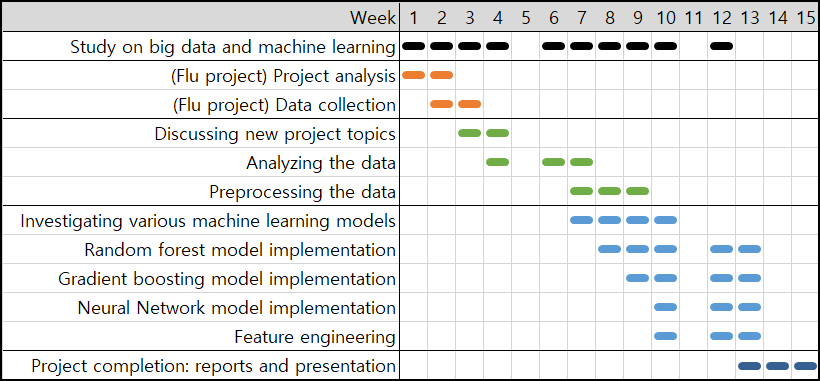
\includegraphics[width=.7\linewidth]{D:/BSG/Desktop/report/gantt2.png}
  \caption{Gantt chart of the works, in weekly basis}
  \label{fig:gantt}
\end{figure}

Note that the introductory week, which is the week before determining the
project to participate, is omitted in the chart. The first week of the project
is the second week of the program(Sep 11$\sim$15), The 14$^{th}$ week of the
project is the 15$^{th}$ week of the program(Dec 11$\sim$15), and so on. Also
note that the week 5 and 11 are the October break and the Thanksgiving break,
respectively.

\newpage
\tableofcontents
\newpage
\section{Introduction}
One of the major recent progresses of the computer science is the machine
learning on big data. It is deeply related to the real life, and they
have synergized with the applications of the artificial intelligence.
Manipulation and analysis on the large amount of data using the machine learning
algorithms allow people approach to problems which are difficult using legacy
methods.

The rapid development of machine learning technology have attracted the managers
in the business area. Companies can enhance their working process and analyze
the behavior patterns of their customers using data they collected. From the
data could have been treated meaninglessly, companies can profit by discovering
its hidden values.

Our team tried to find a problem instance regarding to behavioral pattern of
customers, to stand at the companies' point of view. We joined to the
competition on Kaggle hosted by KKBox(a Taiwanese music hosting company), which
providing enough dataset related to the customers.

\subsection{Aim of the project}
The information of the members, the songs, and the listens(as the train and
the test data) are given in the dataset. We create a prediction
model determining whether the listener would listen that song again within a
month, from the data of listens. The prediction model can estimate the
preference over new songs or artists, eventually provide recommendations to new
users. We use three different models (Gradient Boosting, Neural Network, and
Random Forest) for the prediction and compared their performances.

\subsection{Applications on business area}
For companies, customer specific solutions plays a core role to manage
relationship with the customers, eventually leading to an increase of the
profit.

In this project, predicting the probability of relistens leads to the
extraction of individual preferences. The model also shows the trends of customers listening certain
songs. This encourages the company enhance their music recommendation system
and customized service plans. Through the model, the company can understand
their customers and deploy strategic plans even for their latent customers.
\newpage
\section{Data analysis}
A part of relational database on the company is given as the data to be
analyzed. The CSV-encoded data files are provided for each relevant tables and
columns in the database.

\begin{figure}[!h]
  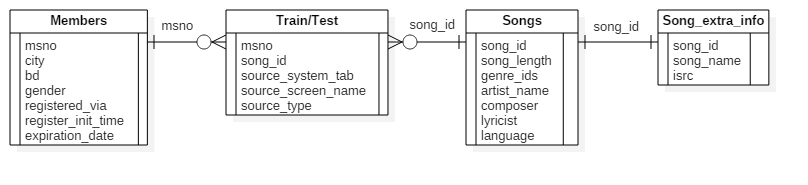
\includegraphics[width=\linewidth]{D:/BSG/Desktop/report/erd.png}
  \caption{Entity-relation diagram of the given data}
  \label{fig:erd}
\end{figure}
\begin{table}[!h]
\centering
\begin{tabular}{|l|l|l|}
\hline \rowcolor[HTML]{C0C0C0}
Data & Meaning & Format \\\hline
msno & Member ID & Hashed Value \\\hline
city & City category & Integer/Nominal \\\hline
bd & Age, in years & Integer \\\hline
gender & Gender & Binary \\\hline
registered\_via & Method of registration & Integer/Nominal \\\hline
registered\_init\_time & Membership registration date & Date \\\hline
expiration\_date & Membership expiration date & Date \\\hline
song\_id & Song ID & Hashed Value \\\hline
song\_length & Length of the song, in milliseconds & Integer \\\hline
genre\_ids & Genre categories & (Integer/Nominal)* \\\hline
artist\_name & Name of the artists & (String)* \\\hline
composer & Name of the composers & (String)* \\\hline
lyricist & Name of the lyricists & (String)* \\\hline
language & Dominant language & Integer/Nominal \\\hline
song\_name & Title of the song & String \\\hline
isrc & ISRC serial number & String \\\hline
source\_system\_tab & Tab name which the song was played &String/Nominal\\\hline
source\_screen\_name & Screen name which the song was played&String/Nominal\\\hline
source\_type & Menu which the song was played & String/Nominal\\\hline
\end{tabular}
\caption{List of the features provided in the dataset}
\label{table:features}
\end{table}

The dataset have several properties important for our analysis.
\paragraph{Categorical data.}
Most features of the data are categorical even they are represented as
numbers. Specifically, they are nominal features rather than ordinal, as the
numbers have no intrinsic orders.
\paragraph{Multiple values.}
Some features including the genre and the artists have multiple values
separated by bars. This indicates that the original database is
a denormalized database from the 1NF.
\paragraph{Incomplete member data.}
Member data including the gender, the age, and the city have much incomplete
data. Especially, approximately 42\% of the members did not provide their age
information; their ages are represented as 0.

\newpage
\section{Neural network}
Artificial Neural Network(NN) is a re-arising method of machine learning, which
mimics the activity on brain cells (neurons). If the states of the input neurons
$x_i$ is given, the output is given by
\begin{equation*}
output = f \left( \Sigma \left( w_i x_i \right) +b \right)
\end{equation*}
where $w,b,f$ represents weights, bias, and an activation function,
respectively.
Weights and biases would be randomly set first, and improved throughout the training, by manually calculating back-propagation formula or just running some optimizations. Such neurons are linked to build a model; layers (groups of neurons) are used for the simplicity.
Recently researchers developed some variants of NNs including Convolutional NN for image recognition and Recurrent NN for serial data analysis. However, as these models assume spatial and temporal locality of input layers, they are not appropriate for this project as the project analyzes separated features. In this project, we used layers of dense networks mainly.
Some python libraries including Tensorflow and Theano aim to support neural networks. We used GPU implementation of Tensorflow for this project.

\subsection{Categorical data preprocessing}
Neurons only accept numbers as the level of activation, making the NN rather
ineffective to deal with categorical data. To use NN with nominal data, we could have following approaches to convert them into numbers.
\paragraph{Binary feature.}
As the gender is a binary feature, it can be directly processed such as (male=1,
female=0). Nulls can be mapped into 0.5, or the portion of males from gender-known members.
\paragraph{Dummy variables.}
Dummy variable(or indicator variable) is a binary variable having 1 or 0,
representing whether some condition is met or not. To encode the categorical
feature into dummy variables, one can introduce columns for each source
categories, and encodes the value as 0 or 1 depend on whether the column indicates the value of source category.

\begin{table}[!h]
\centering
\begin{tabular}{ccc}
\begin{tabular}{|l|l|}
\hline \rowcolor[HTML]{C0C0C0}
ID & Genre \\\hline \rowcolor[HTML]{FFFFFF}
1 & Pop \\\hline
2 & Rock \\\hline
3 & Pop $\vert$ Electronic \\\hline
4 & (null) \\\hline
\end{tabular}
& $\rightarrow$ &
\begin{tabular}{|l|l|l|l|}
\hline \rowcolor[HTML]{C0C0C0}
ID & Genre\_Pop & Genre\_Rock & Genre\_Electronic \\\hline \rowcolor[HTML]{FFFFFF}
1 & 1 & 0 & 0 \\\hline
2 & 0 & 1 & 0 \\\hline
3 & 1 & 0 & 1 \\\hline
4 & 0 & 0 & 0 \\\hline
\end{tabular}
\\
\end{tabular}
\caption{Example of a dummy variable conversion}
\label{table:dummyvariables}
\end{table}
The details how to deal with nulls(ID 4) and multiple values(ID 3) may vary by
methods. If exactly one 1 exists in every records because of absence of
null or multiple values, the table is called a complete disjunctive table(CDT).
Making dummy variables is still one of the simplest methods to encode
categorical variables and becomes the base of other categorical data processing methods.
Large number of distinct categories may lead to the same number of features; one
can use some workarounds such as retaining `Top n' categories.
\paragraph{Multiple Correspondence Analysis(MCA).}
For multiple related categorical variables, MCA converts them to tuples of
numbers, by applying PCA to their CDTs after having some transformations.
If one visualizes the table using the numbers in the tuples as coordinates, he
or she may notice some underlying structures and relationships between the categories.
\begin{table}[!h]
\centering
\begin{tabular}{ccc}
\begin{tabular}{|l|l|l|l|}
\hline \rowcolor[HTML]{C0C0C0}
ID & Source1 & Source2 & Source3 \\\hline \rowcolor[HTML]{FFFFFF}
1 & My Library & My Profile & My Profile more \\\hline
2 & Radio & Radio & Listen to \\\hline
3 & Playlist & Others Profile & Purchase \\\hline
\end{tabular}
& $\rightarrow$ &
\begin{tabular}{|l|l|l|}
\hline \rowcolor[HTML]{C0C0C0}
ID & F1 & F2 \\\hline \rowcolor[HTML]{FFFFFF}
1 & 0.88 & 0.79 \\\hline
2 & 0.22 & 0.17 \\\hline
3 & 0.65 & 0.23 \\\hline
\end{tabular}
\\
\end{tabular}
\caption{Example of a MCA conversion}
\label{table:mca}
\end{table}
\paragraph{Application.}
Note that nominal features other than sources and genres are not used in this
analysis. The features include city, registered\_via, language, and artists; we
expect the performance rise is negligible if we add these features by converting
them into numbers. We only created dummy variables for Top 32 genres and all
source features to use in NNs.

\subsection{Data transformation and normalization}
Experts say that ``In addition to the necessity of encoding categorical data,
experience has shown that neural network training is usually more efficient when
numeric x-data are scaled, or normalized, so that their magnitudes are
relatively similar.''\cite{WEBSITE:NNDataStandardize}
We applied some nonlinear transformations to reflect the property of data or remove
skewness on the data, and adjusted the data to have similar scale (between 0 and
1).
\paragraph{Normalizer.}
Normalizer generates a nonlinear transformation mapping min\_value to 0 and
max\_value to 1.
The function should be an increasing function to obtain meaningful results.
\begin{table}[!h]
\centering
\begin{tabular}{|l|} \hline
def trimmer(x):\\
\hspace{1cm} return 0 if x$<$0 else 1 if x$>$1 else x\\
def normalizer(min\_value, max\_value, func, positive=False, unknown=0.5):\\
\hspace{1cm} return lambda x: unknown if math.isnan(float(x)) or (positive and
x$<=$0) \textbackslash\\
\hspace{2cm} else
trimmer((func(float(x))-func(max\_value))/(func(min\_value)-func(max\_value)))
\\\hline
\end{tabular}
\begin{tabular}{|l|l|l|l|l|}
\hline \rowcolor[HTML]{C0C0C0}
Features & func & min\_value & max\_value & Notes \\\hline
bd (age, yr) & Sqrt & 9 & 49 & Adjusting the mode(25) into 0.5 \\\hline
song\_length (ms) & Log & 32768 & 1048576 & \\\hline
member\_duration (s) & Log & 1 & 444873600 & reg\_init\_time-expiration\_date 
\\\hline
\end{tabular}
\caption{Code and List of the features preprocessed with the normalizer}
\label{table:features}
\end{table}
\paragraph{Decayer.}
Decayer generates an exponential decay transformation when the current
point(which mapped to 1) and the decaying rate(as the half-life) are given.
\begin{table}[!h]
\centering
\begin{tabular}{|l|} \hline
def decayer(current, halflife, unknown=0.5):\\
\hspace{1cm} return lambda x: unknown if math.isnan(float(x)) else 1 if
float(x)$>$current \textbackslash\\
\hspace{2cm} else math.pow(0.5,(current-float(x))/halflife)
\\\hline
\end{tabular}
\begin{tabular}{|l|l|l|l|}
\hline \rowcolor[HTML]{C0C0C0}
Features & current & halflife & Notes \\\hline
song\_year (yr) & 2017 & 10 & Data from isrc \\\hline
registration\_init\_time (s) & 1488258000 & 100000000 & current: Feb 28, 2017
\\\hline
\end{tabular}
\caption{Code and List of the features preprocessed with the decayer}
\label{table:features}
\end{table}

For example, as recent songs have more listens than older ones and the
popularity of songs usually have exponential decay, it is reasonable that we
preprocess the release years of the songs using a decaying function (we chose
half-life 10 years in this case). The decaying function relatively spreads out
the recent song, making the recent songs more distinguishable.

\subsection{Network design}
To examine effects of network modification, we set the different configurations
of the networks. The baseline network is a 3-layered ReLU network with no
dropouts. We changed the number of the neurons and the number of layers, changed
the dropout rates, used the logistic function as the activation function, and
split the inputs to follow different path on the network.

Aside from the shape of the networks, we modified iteration number of trains.
The baseline network uses 50000 steps; we also tried 30000(Train-) and 100000(Train+) steps of trains.
\newpage
\begin{figure}[!h]
  \centering
  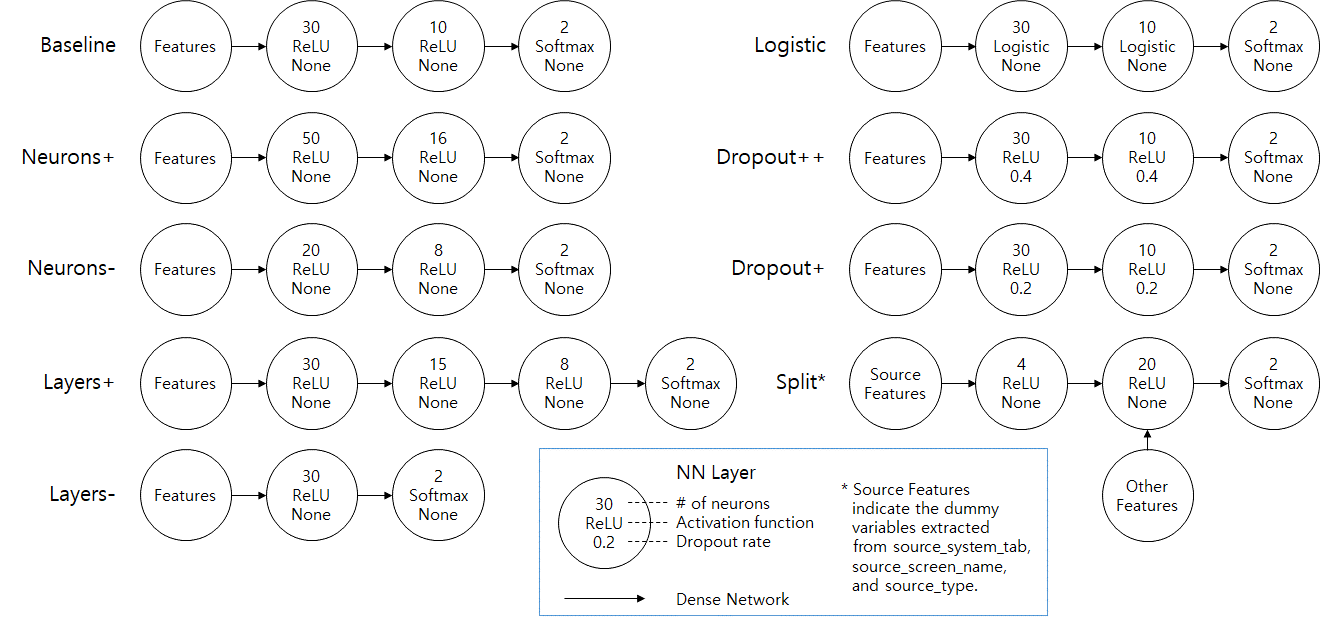
\includegraphics[width=\linewidth]{D:/BSG/Desktop/report/networks.png}
  \caption{Network structures}
  \label{fig:nn}
\end{figure}

\subsection{Results}
As we have expected from ineffectiveness of treating nominal data by NN, the
general results are around 70\% validation accuracy, which is far more
inaccurate than the results of other models.
\begin{figure}[!h]
  \centering
\begin{subfigure}[h]{.50\textwidth}
  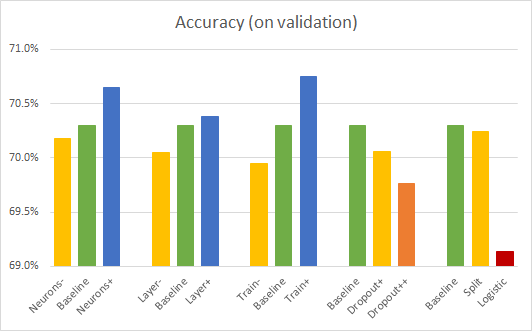
\includegraphics[width=\textwidth]{D:/BSG/Desktop/report/nnaccuracy.png}
  \caption{Network performances in validation accuracy}
\end{subfigure}
\begin{subfigure}[h]{.47\textwidth}
  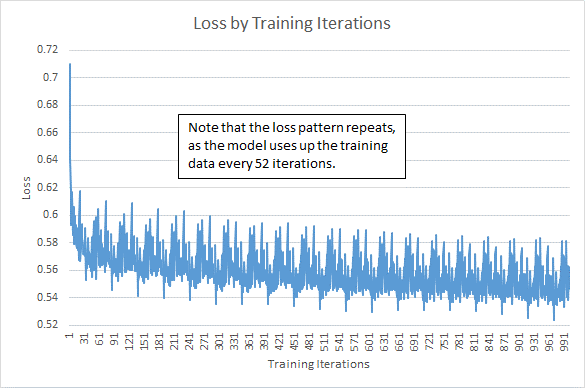
\includegraphics[width=\textwidth]{D:/BSG/Desktop/report/nnloss.png}
  \caption{Loss improvement}
\end{subfigure}
  \caption{Results of NN models}
  \label{fig:nnresult}
\end{figure}

Still, we could observe tendency of accuracy by the model parameters including
number of neurons and the number of layers. While addition of the neurons, the
layers, or the training iterations improves the model as expected, the dropout
technique seems to prevent the models to improve. When we split data and pass it
to different locations of the network separately, the results are better than
Neurons-(28 neurons) and Layers-(30 neurons) models while using only 24 neurons.

It is normal that the score from Kaggle uploads are lower than local validation.
The difference roughly indicates how much the model overfits the data. Upload of
results from Neurons+ model yields 62.172\% score. Compared to validation
accuracy 70.652\%, the difference is roughly 8.5\%p.
Observing the losses during the iterations, we could see decrease of the losses
like the following diagram of Train+ run.

\subsection{Aggregation of multiple networks by voting}
Voting is one of the simplest ensemble methods, letting multiple models to have
multiple predictions and choosing the result which most of the models predicted.
The voting procedure is more effective if the models have similar structures and
produce different predictions due to their different parameters or initial
conditions.\cite{alpaydin1992multiple}

We applied voting to 5 executions of single model (Baseline), and another 5
executions of different models (2 Baselines, Neurons+, Layers+, Split).
It turns out that even the different networks produce similar predictions,
observing that 0- and 5-voted records are dominant. We have 61.262\% submission
score for single model voting, and 61.983\% for different model voting, which is not very different from the original baseline model.
\begin{figure}[!h]
  \centering
  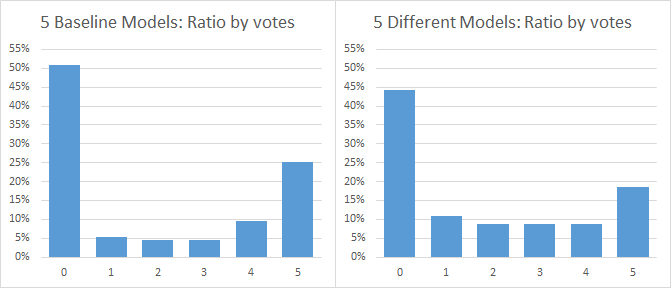
\includegraphics[width=.7\linewidth]{D:/BSG/Desktop/report/votes.png}
  \caption{Distribution of vote results, indicating the number of models
  suggesting the target is 1}
  \label{fig:nnvote}
\end{figure}

\section{Random forest}
\subsection{Bagging}
Random forest is a machine learning algorithm utilizing bagging(bootstrap
aggregating) approach. Bagging is an ensemble method to have votes from
individual models, which uses train data randomly sampled from the whole
train dataset. Two measures, the bias and the variance, have tradeoff
relationship despite they are together the cause of the learning error of a
problem. Bagging can provide an ensemble of models that lowers both measures. To
have an effective result, the underlying models should have high predictability
when the stability is not concerned at all.

\begin{figure}[!h]
  \centering
\begin{subfigure}[h]{.38\textwidth}
  \centering
  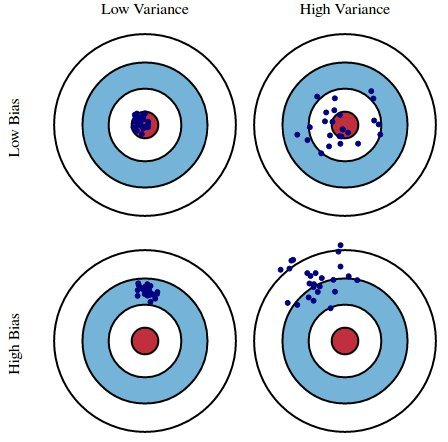
\includegraphics[width=.8\textwidth]{D:/BSG/Desktop/report/bvtradeoff1.png}
  \caption{Diagram of bias and variance\cite[Fig.1]{WEBSITE:bvtradeoff}}
\end{subfigure}
\begin{subfigure}[h]{.60\textwidth}
  \centering
  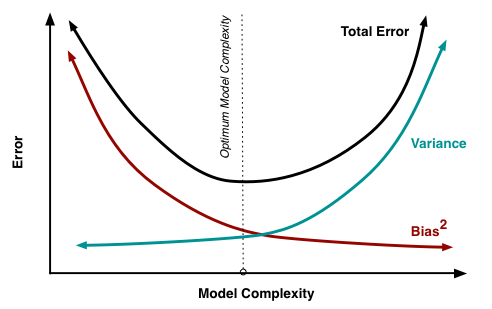
\includegraphics[width=.8\textwidth]{D:/BSG/Desktop/report/bvtradeoff2.png}
  \caption{Bias and variance contributing to total error\cite[Fig.6]{WEBSITE:bvtradeoff}}
\end{subfigure}
  \caption{Bias-variance tradeoff\cite{WEBSITE:bvtradeoff}}
  \label{fig:bvtradeoff}
\end{figure}

\subsection{Decision tree, as the underlying model}
A random forest uses decision trees as the underlying model of bagging.
Decision trees are quite unstable classifiers, but they can effectively deal
with categorical data. Decision trees become less effective if too many features
are given; this is because only one feature should be selected at the each node
and the selected feature is more probably not the best feature. Fortunately, the
effect on the number of features is quite negligible for less than 100 features.

As a random forest behaves like a black box, the flow of logic could be
unexplanatory for humans different from the individual decision tree. However,
it is easy to use because only 3 major hyperparameters are required. The number
of decision trees, the depth of the trees, and the sampling rate for bagging should be provided.

\subsection{Results}
The random forests have around 70\% validation accuracy, which is similar to
the neural networks. However, the properties of bagging can lead the model to
have less overfitting. The prediction accuracy is around 65\%, which provides
accuracy difference near 5\%p which is the smallest among the models we used.

\section{Gradient boosting}
A gradient boosting model(GBM) is a group of gradient descent models ensembled
with boosting method. Boosting is a serial ensemble method which gradually
increases weight of misclassified data. Originally the gradient descent models
modifies parameters by calculating the gradient of the loss function through
partial derivation, multiplied by the specified learning rate $\alpha$.
\begin{equation*}
\mathbf{v}_{new} = \mathbf{v}_{old} - \alpha \bigtriangledown Loss \left( \mathbf{v}
\right)
\vert_{\mathbf{v}_{old}}
\end{equation*}

GBM applies the gradient of the loss function for the whole parameters
used in partially aggregated model learned so far. GBM requires the learning
rate, the loss function, and the parameters for the boosting(such as the number
of models) as its hyperparameters.

\subsection{Data preprocessing and feature engineering}
For the null or invalid values, they are replaced into average value of the
feature in case of numeric features(including song\_length), or a category
indicating the absence of the values in case of categorical feature. The
data types of each of the feature columns are stated explicitly.

Feature engineering is a preprocessing procedure which extracts new
features can be considered meaningful, from the existing features. We extracted
some temporal aspects of the features separately, such as year/month/day of date
features and release year from the ISRC codes. The numbers of song plays by
songs or artists are added. The length of the songs are categorized by equally
ranged group using the half of the average length as the size of the ranges.

\begin{table}[!h]
\centering
\begin{tabular}{|l|l|l|}
\hline \rowcolor[HTML]{C0C0C0}
Steps & Introduced Feature & Prediction accuracy \\\hline
1 & Using features only occuring in the provided data & 62.0\% \\\hline
2 &	Stating the explicit types of the columns & 62.8\% \\\hline
3 & Extracting release years of the songs from ISRC & 64.2\% \\\hline
4 & Separating dates into year, month, and day & 65.6\% \\\hline
5 & Adding the number of artists, composers, and lyricists & 66.8\% \\\hline
6 & Categorizing the song length & 67.6\% \\\hline
7 & Adding the numbers of song plays by songs & 68.3\% \\\hline
8 & Adding the numbers of song plays by artists & 68.7\% \\\hline
\end{tabular}
\caption{List of the features provided in the dataset}
\label{table:gbmfeatureengineering}
\end{table}

\subsection{Results}
We used LightGBM library provided by Microsoft. As we introduced features from
the feature engineering procedures, the prediction accuracy continues to improve if the features are effective.

\begin{figure}[!h]
  \centering
  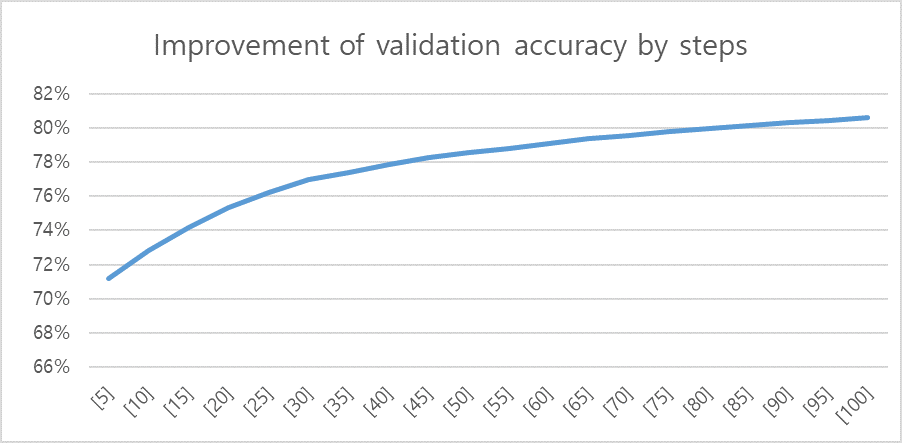
\includegraphics[width=.5\linewidth]{D:/BSG/Desktop/report/gbmimprove.png}
  \caption{Improvement of validation accuracy throughout the training}
  \label{fig:gbmimprove}
\end{figure}

The final model(learning rate 0.2, 100 boostings) produces 68.71\% prediction
accuracy, and its corresponding validation accuracy is 80.6\% for the best model. Though the difference(12\%p)
which is the largest among the models shows large degree of overfitting, the
prediction accuracy is the best result we could obtain so far.
Adding more features lead to the memory overflow error in the laptops, limiting
the number of features we could actually use.

\section{Conclusion}
We attempted to produce a solution for prediction problem using the three(Random
Forest, Gradient Boostring, Neural Network) machine learning models. We could
have following accuracy results.
\begin{figure}[!h]
  \centering
  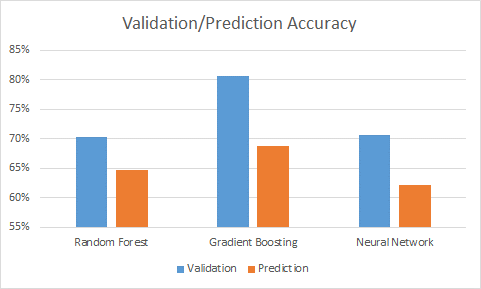
\includegraphics[width=.6\linewidth]{D:/BSG/Desktop/report/result.png}
  \caption{Validation and prediction accuracy of each models}
  \label{fig:result}
\end{figure}

Comparing these models one another, GBM has the best prediction accuracy. Random
forest shows the lowest overfitting(difference of the two accuracy values)
rates. Neural Network is the least accurate model as the categorical data is the predominant
feature type of this problem.

All members in our team started the project without the background knowledge
about machine learning. Though it is not the best result in the competition,
this was a fine opportunity to deal with various kinds of data and models. We
learned the underlying theories and details of models, and got intuition about
data relationship and preferred analysis method by trials and errors.

It is interesting that we analyzed the data used in actual business area, while
maintaining competitive relationship with the other teams in the competition.
This kind of experience would be a substantial help when we advance into
the actual business area in the future.

\newpage
\begin{appendices}
\section{Weekly tasks of the project}

\begin{table}[!h]
\centering
\begin{tabular}{|l|l||l|l|}
\hline \rowcolor[HTML]{C0C0C0}
W. & Task & W. & Task \\\hline \rowcolor[HTML]{FFFFFF}
0 & Introduction and project determination & 8 & Started RF and data
preprocessing \\\hline
1 & Introduction to big data and the flu project & 9 & Started GBM and parameter
tuning
\\\hline
2 & Data collaction for the flu project & 10 & Started NN using
Tensorflow-GPU
\\\hline
3 & Topic pivoting to music relisten prediciton & 11 &
Thanksgiving break \\\hline
4 & Analysis of the given data & 12 & Feature engineering
\\\hline
5 & October break & 13 & Improving models using the new features
\\\hline
6 & Validating hypotheses on data correlation & 14 & Project wrap-up and
writing reports \\\hline
7 & Investigation on categorical data analysis & 15 & Preparing the
final presentation \\\hline
\end{tabular}
\caption{Weekly tasks of the project}
\label{table:weektask}
\end{table}

\section{Work contribution}
Our team has a democratic team structure providing equal relationship among the
five teammates. The team is driven by ourselves; we decided our own goals under
some advice from Assoc. Prof. John A. Springer. Though we had no firm work
distributions except for each models, we had helped one another through
suggestions based on goals we discussed in each weeks. The following describes
the major contributions of the each team members.

J.Bae and J.Kang together concentrated on Gradient boosting and
feature engineering, producing the best result among our trials. S.Baek focused
on Neural networks while also concerning team management and some data
preprocessing. Y.Jang aimed on Random forests and tried to seek and crawl
external relevant data earlier in the project. N.Kim played the key role on
designs of the documents and the presentation, also putting her effort on
literature search.

The final presentation is mainly done by J.Kang and N.Kim. J.Bae, S.Baek, and
Y.Jang contributed to the contents of the report. S.Baek wrote this report in
English refining the original report in Korean.

\section{Notes on project topic change}
The flu spreading model is a major research accomplishment of the project
advisor, Prof. John A. Springer. The first topic we selected was to apply the
flu spreading model, in Korea, using various sources of the data.

We had made attempt to collect the necessary data including weather data,
medical data, and the social media data. Weather data could be easily acquired
through Korea Meteorological Administration. For the social media data, the
users rarely allow their location to be posted; some media do not provide
their API public. Especially for the medical data, no suitable data is
available to use. A cohort sample with a million anonymized patients is not
only expensive, but also not a real-time data. Offices of education
monitor the students with flu and upload their report online every week; it is
the data with best temporal granularity, but the data is in document form and
only students are monitored. There are no data sources with the spatial
granularity finer than the province level.

Meanwhile, National Health Insurance Service(NHIS) in Korea already have
prediction models for various diseases, provided to the public through 'Public
health Alarm Service'.
Though flu is not directly included in the service, the service predicts cold. As NHIS have
its own real-time medical data we cannot obtain, it is capable to provide
accurate predictions, different from our team. We decided to find a new project topics
which data is available to use.
\end{appendices}
\newpage
\paragraph{Acknowledgement.}
This project is a result of Korea Software Square 2017 Capstone 8 program
organized by IITP and Purdue University. We appreciate to the project advisor Prof. John
A. Springer and the program manager Prof. Eric T. Matson, making our projects to
be more successful. We also appreciate to IITP and each universities the
team members are belonging to, for the support and the funding to this program.
\nocite{ARTICLE:breiman2001random,LECTURE:BaggingRF,MANUAL:LightGBMDoc}
\bibliography{document} 
\bibliographystyle{ieeetr}
\newpage
\section*{Opinions and suggestions}
\paragraph{On government-driven public open data system in Korea.}
As my team gave up the original topic of the project due to the lack of data, I
have some thoughts on public data provided by the government.

It is nice that the Korean government manages the portal on public
data(www.data.go.kr), which collects many sources of the data provided by the
government. Each websites of government offices and government-related
public enterprises also provide their data. However, many aspects of the data
cause some inconvenience to the people who want to utilize the data.

\subparagraph{Access Control.}
The appropriate level of the government's access control on
public data is often disputable, which could be a political problem. However, it is obvious
that for the transparency of the government, the activity and aspects of the
government should remain public as much as possible unless it cause some
security threats or infringe rights of some legal entities.

In many government-driven systems of public data, users are required to sign
up(which means providing personal information) and often write
the purpose to access to the data for the approval. Though it is not a
barrier for people who want to access to the data in the systems with
automatic approvals, it is still one of the forms of data access control by
government.

\subparagraph{Cost of data sell.}
Public enterprises often `sell' the access rights to their data to
researchers. For example, National Health Insurance Service(NHIS) sells the
access right to a dataset of 1 million anonymized sample of medical records
(called a medical cohort) in 25,000 won per day. A person should work 3 hours
and 52 minutes a day in the minimal wage of 2017, just to maintain the access to
the dataset.

Though public enterprises could charge money for data access as they are also
enterprises that pursue profit, the cost should be reasonable considering the public aspects of the data.

\subparagraph{Real-time update.}
Data providers are expected to keep
the data up-to-date. However, the government, which is the provider of many
public data, does not. Many datasets are outdated over an year; even the
expensive medical cohort is made from samples on 2002 to 2013.
Analysts and decision makers cannot predict the recent trends accurately using
outdated data produced long ago.




\end{document}
